%%
%% This is file `article1.tex', % generated with the docstrip utility.
%%
%% The original source files were:
%%
%% dms.dtx  (with options: `article') % Example TeX file for the documentation %
%of the jurabib package % Copyright (C) 1999, 2000, 2001 Jens Berger % See
%dms.ins  for the copyright details.
%% 
%%% ====================================================================
%%%  @LaTeX-file{ %%     filename        = "dms.dtx", %%     author    =
%"Nicolas Beauchemin, Damien Rioux-Lavoie, Victor Fardel, Jonathan Godin", %%
%copyright = "Copyright (C) 2000 , DMS %%                  all rights reserved.
%Copying of this file is %%                  authorized only if either: %%
%(1) you make absolutely no changes to your copy, %%                  including
%name; OR %%                  (2) if you do make changes, you first rename it %%
%to some other name.", %%     address   = "Département de Mathématiques et de
%Statistique", %%     telephone = "514-343-6705", %%     FAX       =
%"514-343-5700", %%     email     = "aide@dms.umontreal.ca (Internet)", %%
%keywords  = "latex, amslatex, ams-latex, theorem", %%     abstract  = " Ce
%fichier est un package conçu pour être %%                  utilisé avec la
%version de LaTeX2e 1995/06/01. Il %%                  est prévue pour la classe
%``amsbook''. Il en %%                  modifie le format des pages, l'entête
%des %%                  sections, etc, afin d'être  conforme au modèle de %%
%mémoire de maîtrise de l'Université de %%                  Montréal. Finalement
%ce fichier est grandement %%                  inspiré du fichier
%amsclass.dtx.", %%     docstring = "The checksum field contains: CRC-16
%checksum, %%                  word count, line count, and character count, as
%%%                  produced by Robert Solovay's checksum utility."}
%%%  ====================================================================


%% To change chapter header dynamically from french to english, use
%%\entetedynamique
\setcounter{corA}{0} % Pour recommancer à compter les def,
                     % theo, etc. à partir de 1
 % Pour écrire un article en français
%% \francais
 % Pour écrire un article en anglais
\anglais
%% NOTE: La plupart des macros ont un nom en anglais. % P.ex. \adresse et
%\address fonctionnent et sont équivalents. % \revue=\journal % \auteur=\author
%% \titre=\title

\doublespacing

%% Les contributions apparaîtront habituellement après % \maketitle (voir un peu
%plus bas). Selon les goûts, il est % possible de mettre les contributions %
%avant la page titre de l'article, simplement en les écrivant % directement ici.
%Par exemple :
 % \cleardoublepage \pdfbookmark[chapter]{Contributions}{contrib1} % Remplacer
 % par contrib2 pour l'article 2 etc. {\bfseries\Large\noindent Contributions de
 % <mon nom> et rôle joué par les coauteurs} J'ai contribué en...
 %
 % Le rôle des coauteurs a été de...

%% Nom de la revue de publication
\revue{Ecography and can be found at https://doi.org/10.1111/ecog.06609}
\article{SpatialBoundaries.jl: Edge detection using spatial wombling}\label{SpatialBoundaries}
%% On peut se référer aux numéros de chapitre ou d'article comme suit. % Si on
%fait % \label{chap:article1}, % alors \ref{chap:article1} donnera le numéro du
%chapitre. On peut ensuite faire % \labelart{art:article1} % et alors
%\ref{art:article1} donnera le numéro d'article. % Par exemple, si cette article
%est le premier article et le deuxième chapitre, % alors si on écrit % Voir le
%chapitre~\ref{chap:article1} (l'article~\ref{art:article1}). % deviendra % Voir
%le chapitre 2 (l'article 1). % Si on veut écrire « premier article » au lieu «
%article 1 », on peut % simplement faire % \ordinal{\ref{art:article1}}~article
%% devient première article % ou % \Ordinal{\ref{art:article1}}~article  %
%devient Première article (avec la majuscule) % Si on est en mode \anglais,
%\ordinal écrire first, second,...

%%%%%%%%%%%%%%%%%%%%%%%%%%%%%%%%%%%%%%%%%%%%%%%%%%%%%%%%%%%%%%%
%%%%%%%%%%%%%%%%%     Contribution     %%%%%%%%%%%%%%%%%%%%%%%% %%%%%%%%%%%%%%%%
%(lire attentivement) %%%%%%%%%%%%%%%%%%%%%%%%
%%%%%%%%%%%%%%%%%%%%%%%%%%%%%%%%%%%%%%%%%%%%%%%%%%%%%%%%%%%%%%%
 % Contribution(s) peronnelle(s) à l'article et rôle joué par tous les
 % coauteur·e·s
 %
 % Nécessaire seulement lorsque vous n'êtes pas seul·e auteur·e. Les
 % contributions peuvent apparaître ailleur dans la thèse. Si \contributions est
 % laissé vide (p.ex. si vous effacez celui ci-bas), aucune contributions ne
 % seront générées sur la page titre de l'article. Vous pouvez alors mettre un
 % \newpage si vous souhaitez que les résumé et abstract soient sur la page
 % suivante.
 %
 % REMARQUE : À peu près toutes les constructions \LaTeX\ sont permises dans les
 % contributions.
 %
 % La commande admet une option [<entête>]
\contributions%[Mes contributions et le rôle des coauteurs]
{ TP and TS designed the study and developed the software. TS was the lead on writing and editing.\\[1cm]
}

%%% INFORMATIONS POUR LA PAGE TITRE
 % Premier auteur·e et adresse

\auteur{Tanya Strydom}
\adresse{Département de Sciences Biologiques, Université de Montréal, Montreal, QC, Canada\\ Québec Centre for Biodiversity Sciences, Montreal, QC, Canada}
\auteur{Timothée Poisot}
\adresse{Département de Sciences Biologiques, Université de Montréal, Montreal, QC, Canada\\ Québec Centre for Biodiversity Sciences, Montreal, QC, Canada}
%

\maketitle
\begin{refsection}

\begin{resume}{wombling spatial, détection des contours, limites, écologie spatiale, logiciel, Julia} Le wombling spatial est une approche permettant de détecter les contours d’un paysage bidimensionnel défini. Ceci est réalisé en calculant le taux et la direction du changement grâce à l’interpolation de points. Cela donne non seulement une approximation de la forme du paysage, mais peut également être utilisé pour identifier des cellules de limites potentielles qui délimitent un passage d'un état à un autre au sein du paysage. Nous présentons ici le package SpatialBoundaries.jl pour Julia, qui a été développé pour implémenter l'algorithme de wombling pour les ensembles de données référencés spatialement pour des paysages échantillonnés de manière uniforme ou aléatoire. D'un point de vue pratique, la fonctionnalité de wombling permet à l'utilisateur de répondre à deux questions: dans quelle mesure et dans quelle direction la variable d’intérêt change-t-elle ? et la fonctionnalité de limites identifie des cellules limites candidates. Nous concluons en fournissant un exemple fonctionnel du package utilisant les différentes couches de plantes ligneuses pour la Grande-Bretagne et l'Irlande à partir de la base de données EarthEnv.
\end{resume}

\begin{abstract}{spatial wombling, edge detection, boundaries, spatial ecology, software, Julia} Spatial wombling is an approach for detecting edges within a defined two-dimensional landscape. This is achieved by calculating the rate and direction of change through the interpolation of points. This not only gives an approximation as to the shape of the landscape but can also be used to identify candidate boundaries cells that delimit a shift from one state to another within the landscape. Here we introduce the SpatialBoundaries.jl package for Julia, which has been developed to implement the wombling algorithm for datasets that are spatially referenced for both uniformly or randomly sampled landscapes.From a practical perspective, the wombling functionality allow the user to answer two questions: how much and in which direction does the variable of interest change? and the boundaries functionality identifies candidate boundary cells. We conclude by providing a working example of the package using the various woody plant layers for Britain and Ireland from the EarthEnv database.
\end{abstract}

\section{Background}\label{background}

There is value in being able to identify boundaries within a landscape
as it provides us with a starting point from which to understand changes
in species assemblages, ecological communities, or even simply to
delineate areas (based on a shared property) into discrete units, for
example ecosystemic regions (\cite{Post2007ProBou, Fortin2000IssRel}).
Here we present a \texttt{Julia} (\cite{Bezanson2017Julia}) package aimed
at detecting boundaries across a specified geographical area by
identifying zones of rapid change using the wombling edge detection
algorithm. This approach was originally developed by \cite{Womble1951DifSys}
in the context of understanding trait variation within a geographic area
and was later modified by \cite{Barbujani1989DetReg} for the purpose of
understanding changes in gene frequencies, although it also has a more
general ecological application with regards to spatial data
(\cite{Fortin2005SpaAna}), serving as a complimentary approach to cluster
analysis (\cite{Fortin1995DelEco}). Wombling has applicability to a wide
range scenarios \emph{e.g.,} trait measurements or genotypes
(\cite{Barbujani1989DetReg}), species interaction networks
(\cite{Fortin2021Network}), and has explicitly been used (to list a few
examples) to detect transitions within a landscape
(\cite{Philibert2008SpaStr, Camarero2000BouDet}), and analyse the spread
of invasive species (\cite{Fitzpatrick2010EcoBou}). Although the origins
of wombling may be rooted in anthropology and has been extensively used
in ecology the potential applicability also extends to other systems
such as high-energy experiments in physics (\cite{Matchev2020FinWom}), or
to understand the genetic-linguistic patterns of European populations
(\cite{Sokal1990GenLan}).

Broadly speaking spatial wombling is an edge-detection algorithm which
traverses a geographic area (for the purpose of this discussion let's
imagine a spatially referenced dataset pertaining to species richness
for each location) and defines this area in terms of the rate ($m$)
and corresponding direction of change ($\theta$) through interpolating
between nearest neighbours. Although the wombling algorithm (as
implemented here) is designed to work with two-dimensional \emph{i.e.,}
planar data (as delimited by $x$ and $y$ --- which would be the
co-ordinates of where species richness was sampled), it is beneficial to
view this plane as a three-dimensional object (or series of curves), as
shown in \autoref{fig:concept_womble}, panel A. Here the `amplitude' of the curvature of
the plane is determined by the value of $z$ (species richness) and the
rate and direction of change is calculated by using the first-order
partial derivative $\partial$ of the surface (curve) as described by
$f(x,y)$. This then gives us an indication of how steep the
gradient/curve ($m$) is between neighbouring cells as well as the
direction (from the `low' to the `high' point; $\theta$) of the slope
(panel B, \autoref{fig:concept_womble}). Large values of $m$ are associated with zones
of rapid change in the landscape and are indicative of a shift from one
`state' to another \emph{i.e.,} a potential ecological boundary within
the landscape (\cite{Fortin2005SpaAna}; dashed line in panel C,
\autoref{fig:concept_womble}). One benefit of the wombling approach is that
interpolation is not necessarily restricted to a rectangular
($2 \times 2$) window (that would entail a landscape where points are
regularly arranged in space) and can easily be re-written so as to
accommodate points that are not regularly arranged across space (as per
\cite{Fortin1994EdgDet}), thereby giving the user more flexibility with
regards to how the sampling points are arranged (\emph{i.e.,} sampled)
across the landscape.

\begin{figure}[h]
    \centering
    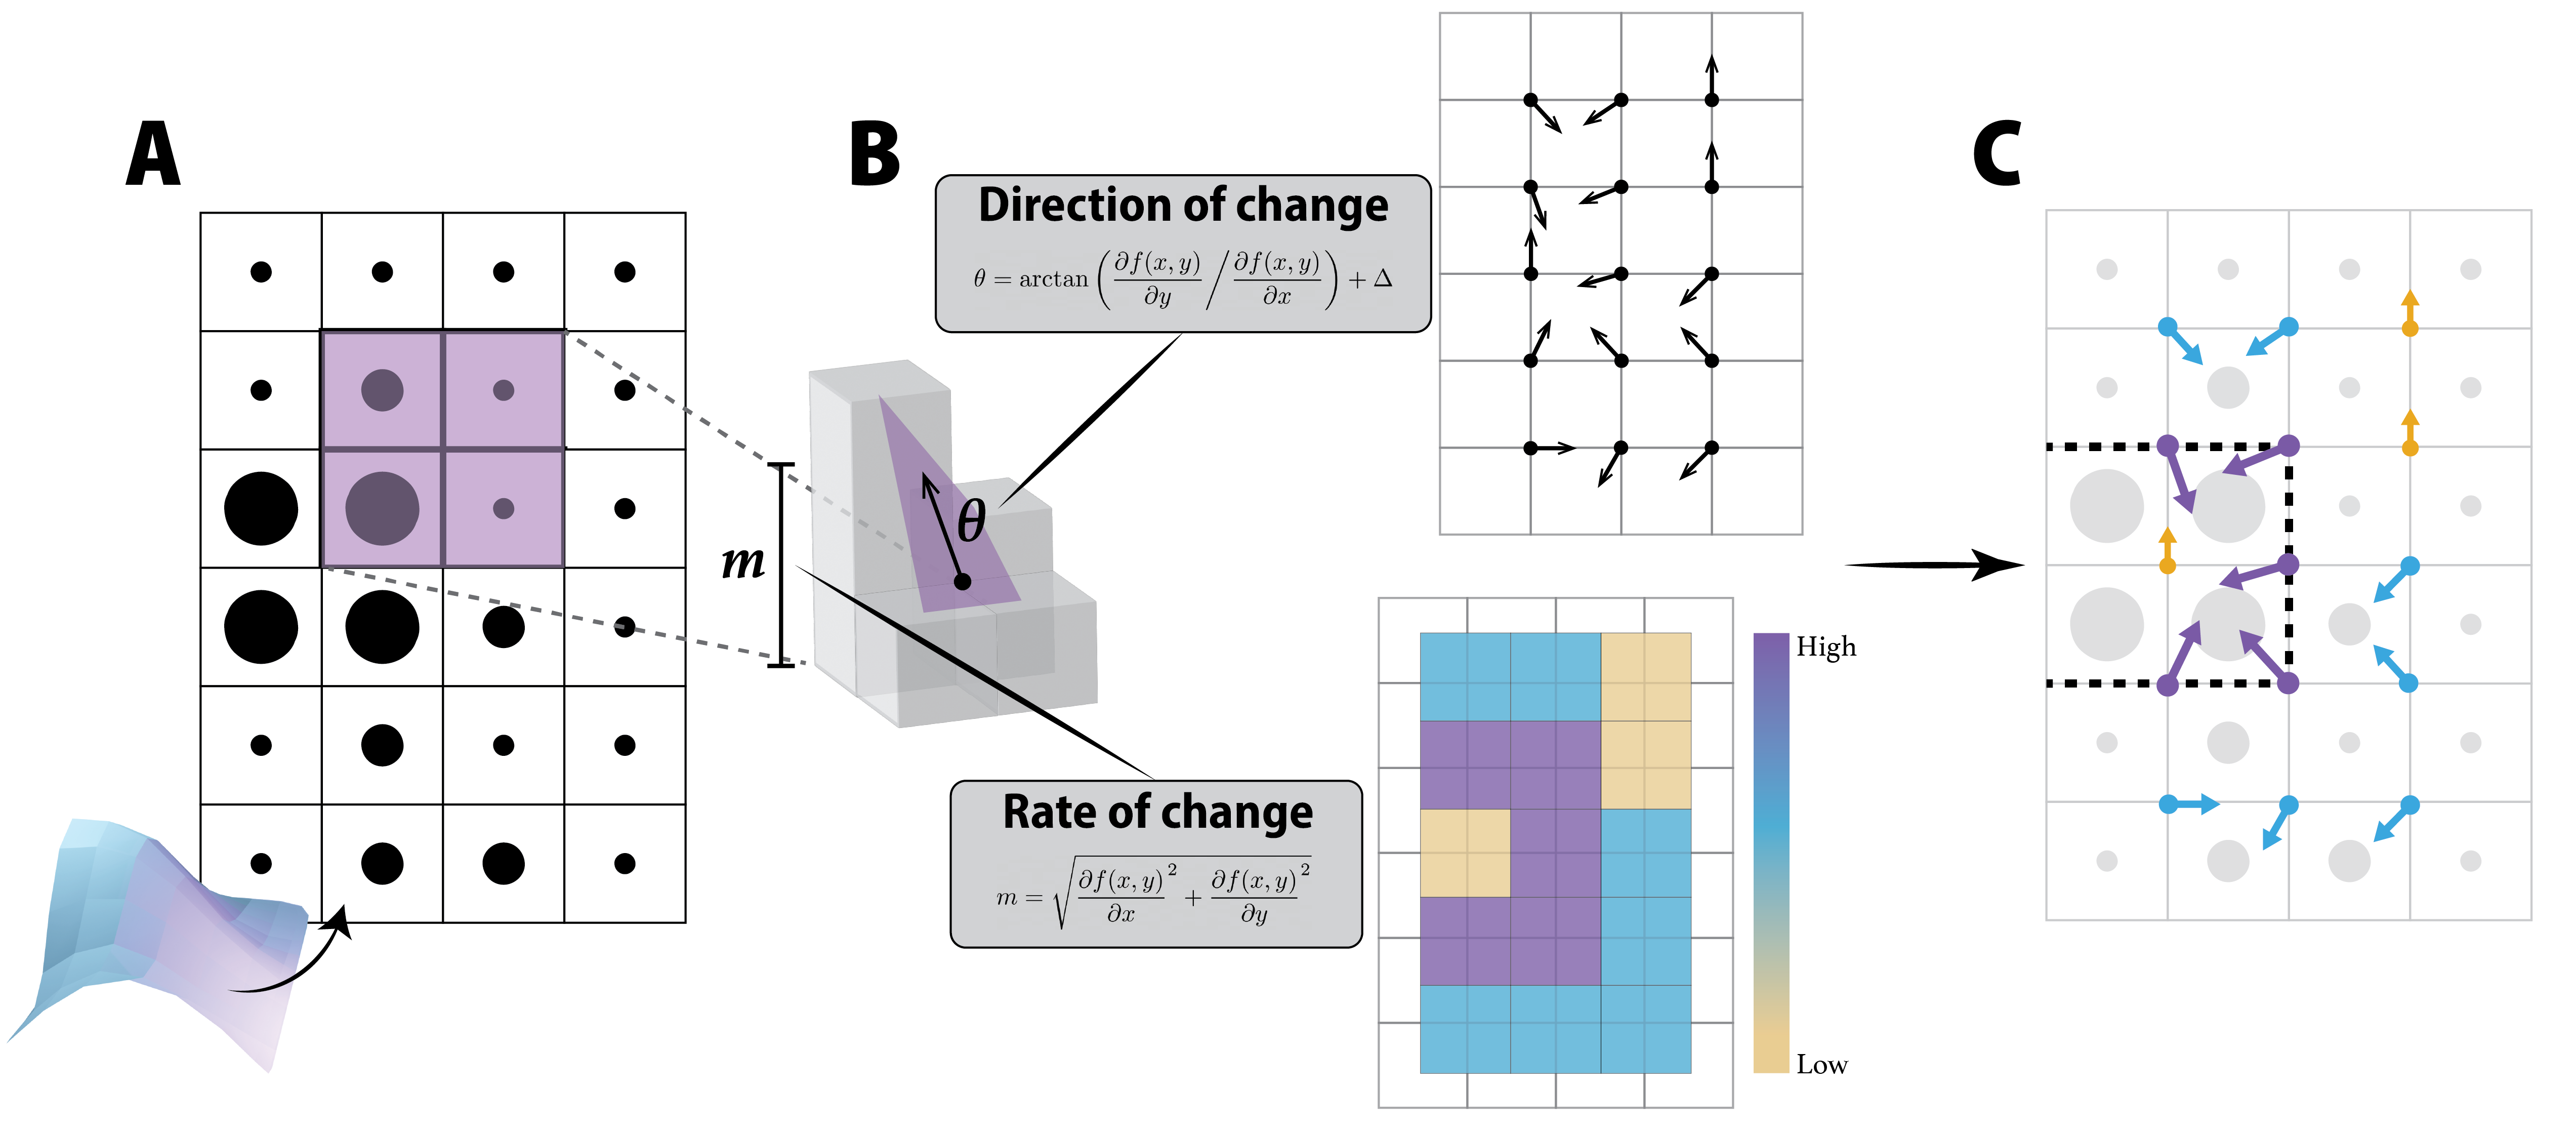
\includegraphics[width=\textwidth]{figures/fig_concept.png}
    \caption{A visual conceptualisation of how the wombling algorithm
interpolates points across a geographical area (in this case the points
are regularly arrange in space) for a variable of interest (\(z\)) to
calculate the rate ($m$) as well as the direction ($\theta$) of
change. Here the sampled landscape is shown in panel A with the size of
the points correlating to the magnitude if the variable of interest
($z$). Panel B shows the two components of the landscape once wombled,
which are then combined and superimposed across the original landscape
in panel C, with the dashed line indicating a candidate boundary. Here
the colours as well as the size of the arrows indicate the rate of
change and the direction should be interpreted as moving from the `low'
to the `high' point. Note that the dimensions of the wombled landscapes
(B) will be smaller than the original landscape (A) due to the
interpolation process \emph{i.e.,} where we originally had an
\(n \times r\) grid we now have an (\(n\) - 1)(\(r\) - 1) sized
grid.}
    \label{fig:concept_womble}
\end{figure}

\subsection{Rate of change}\label{rate-of-change}

The rate of change ($m$) can be used to find the zones of rapid change
within the geographical area --- which, in turn, can be used to identify
potential candidate boundaries. The rate of change is calculated as
follows:

\begin{equation} \label{eq:1}
m = \sqrt{\frac{\partial f(x,y)}{\partial x}^2 + \frac{\partial f(x,y)}{\partial y}^2}
\end{equation}

Where \(f(x,y)\) can be expanded as:

$$f(x,y) = z_{1}(1-x)(1-y) + z_{2}x(1-y) + z_{3}x y + z_{4}(1-x)y$$

For convenience the values of the centroid of the `search window'
\emph{i.e.,} \(x\) and \(y\) can be standardised to 0.5 when working with
points regularly arranged in space. Additionally, as we are
interpolating between points, it should also be noted that the original
\(n*r\) geographical area will now be an \((n -1)(r - 1)\) sized grid
(\emph{i.e.,} one less row and one less column of values for the wombled
landscape as illustrated in panel C of \autoref{fig:concept_womble}).

When we are working with points that are irregularly arranged within the
geographical area it is possible to use triangulation wombling
(\cite{Fortin2005SpaAna, Fortin2021Network, Fortin1994EdgDet}). Here the
approach to wombling has been modified by \cite{Fortin1992DetEco} so as to
interpolate the plane between the three nearest neighbours (as opposed
to the usual \(2 \times 2\) grid). Nearest neighbours are found by using
the Delaunay triangulation algorithm (\cite{Delaunay1934SphVid}) after
which the rate of change is still calculated in the same manner as in
\autoref{eq:1}, however as we are now only working with a three-point
`window' \(f(x,y)\) will be defined as:

$$f(x,y) = ax + by + c$$

where

$$\left[ \begin{array}{ccc} a & b & c \end{array} \right] = 
\left[ {\begin{array}{ccc}
   x_{1} & y_{1} & 1\\
   x_{2} & y_{2} & 1\\
   x_{3} & y_{3} & 1\\
  \end{array} } \right]^{-1}\cdot
  \left[
  \begin{array}{ccc} z_{1} & z_{2} & z_{3} \end{array} \right]$$

and the \(x\) and \(y\) co-ordinates of the centroid of the triangle
formed by the three points are calculated as follows:

$$ \Big( \frac{x_{1} + x_{2} + x_{3}}{3} \Big), \Big( \frac{y_{1} + y_{2} + y_{3}}{3} \Big) $$

\subsection{Direction of change}\label{direction-of-change}

It is also possible to calculate a corresponding direction (\(\theta\))
for each rate of change (noting that the same equation can be used for
both lattice and triangulation wombling). This is calculated as:

$$\theta = \arctan \left( \frac{\partial f(x,y)}{\partial y} \bigg/ \frac{\partial f(x,y)}{\partial x} \right) + \Delta$$

$$\text{where} \quad \Delta =
\left\{ \begin{array}{ccc}
    0 \degree & \text{if} & \frac{\partial f(x,y)}{\partial x} \geq 0 \\
    180 \degree & \text{if} & \frac{\partial f(x,y)}{\partial x} < 0 \\
\end{array} \right\}$$

This gives the direction of change which, as the name implies, indicates
the direction the rate of change is `travelling'. The direction of
change should be interpreted as wind direction \emph{i.e.,} where the
change is coming from and not where it is moving towards. As is the
nature of maths when the rate of change is zero it is still possible to
calculate a \emph{real} direction for the non-change --- which will be
180$^{\circ}$. This means it is possible to think of and use the
direction of change independently of calculating boundaries \emph{per
se} and can be used to inform how the landscape is behaving/changing in
a more `continuous' way as opposed to discrete zones/boundaries. For
example if changes in species richness are more gradual (rate of change
is near constant) but the the direction of change is consistently East
to West (\emph{i.e.,} 90$^{\circ}$) we can still infer that species
richness is more or less uniformly increasing in a South-North direction
(this is somewhat exemplified in the direction of change landscape of
panel B in \autoref{fig:concept_womble} where the dominant direction of change is
East-West).

\subsection{Candidate boundaries}\label{candidate-boundaries}

Detecting boundaries \emph{i.e.,} areas where the angle of the landscape
transitions sharply is surprisingly simple. After having calculated the
rate of change (\(m\)) for the geographical area it is possible to use
these values to identify and assign potential boundaries
(\cite{Fortin2005SpaAna, Oden1993CatWom, Fortin1995DelEco}). As large
rate of change values are indicative of a steep gradient it stands to
reason that these points are indicative of a shift from one state to
another \emph{i.e.,} indicative of a boundary. Following the approach
outlined in \cite{Fortin2005SpaAna} a threshold value (or percentile class)
can be set and will determine what proportion of cells will be retained
as potential boundaries. For example if using a 0.1 threshold then the
highest 10\% of points (which are ranked based on \(m\)) will be
classified as candidate boundaries. Note that points with the same rate
of change will be assigned the same rank meaning that more than 10\% of
the \((n -1)(r - 1)\) could potentially be identified as candidate
boundary cells. This approach to identifying potential boundary cells is
not the sole approach and there are other ways and nuances from which to
approach boundary estimation, such as the use of Voronoi tessellations
(\cite{Fortin1995DelEco, Oden1993CatWom, Matchev2020FinWom}).

\section{Methods and features}\label{methods-and-features}

\texttt{SpatialBoundaries} v0.0.3 implements the Wombling algorithm
within the \texttt{Julia} ecosystem and is made available under the
permissive MIT license. The source code (along with more extensive
documentation) can be found at
\url{https://poisotlab.github.io/SpatialBoundaries.jl/}. This is an open
project and is thus open to contributions. The package itself has two
main functions 1) calculate the rate (\(m\)) and direction (\(\theta\))
of change for landscapes for points that are both regularly (\emph{i.e.,}
lattice wombling) and irregularly arranged cross space (triangulation
wombling) arranged in space using the \texttt{wombling} function (for
which layers can also be aggregated using \texttt{mean}), and 2)
identifying candidate boundary cells based on a user defined threshold
value using the \texttt{boundaries} function. Objects that have been
passed through a wombling function are of the \texttt{Womble} abstract
type (which has the two sub-types of \texttt{LatticeWomble} and
\texttt{TriangulationWomble}). This package is, to the best of our
knowledge, the only package to implement the Wombling algorithm within
\texttt{Julia}.

\subsection{Wombling}\label{wombling}

The \texttt{wombling} function calculates and outputs both the rate
(\(m\)) and direction (\(\theta\); where the direction is denoted from
the `low' to the `high' point) of change for a given geographical area.
Leveraging the multiple dispatch within \texttt{Julia} this one function
will execute either the lattice or triangulation wombling algorithm
depending on the structure (spatial referencing) of the input dataset,
meaning that it does not need to be user specified. When a \emph{matrix}
of \(z\) values is used (where the row and column id's act as the
co-ordinates) the lattice wombling algorithm will be executed and when
three \emph{vectors} (consisting of the co-ordinates (\(x\) and \(y\)),
and \(z\) values respectively) the triangulation wombling algorithm is
executed. The resulting output object will have two components (\(m\)
and \(\theta\)) and will be typed based on the wombling method used.
That is a uniform matrix will result in an object of the type
\texttt{LatticeWomble} and irregularly arranged points will be of the
type \texttt{TriangulationWomble}.

\subsection{Overall mean wombling
value}\label{overall-mean-wombling-value}

The \texttt{mean} function calculates the Overall mean wombling value.
The methodology stems from the Overall Mean Lattice-Wombling Value
(\(\bar{m}\)) used by \cite{Fortin1994EdgDet} in which multiple surfaces
(think different \(z\) variables) can be overlaid for the purpose of
finding the mean rates and directions of change for a composite
landscape. The mean rate of change can be defined as the average of
\(m\) values (for a specific centroid) for the given set of surfaces and
the same is done for the direction of change using the \(\theta\)
values. Alongside the mean the standard deviation is also calculated for
both the rate and direction of change. Although \cite{Fortin1994EdgDet} only
present this approach for lattice wombled landscapes we have extended
the functionality to include both lattice and triangulation wombled
types. This is provided that the landscape (\emph{i.e.,} co-ordinates) of
the different surfaces are \emph{exactly} the same. Note here that the
original wombling type is retained and the output data will remain
either type \texttt{LatticeWomble} or \texttt{TriangulationWomble}.

\subsection{Boundaries}\label{boundaries}

The \texttt{boundaries} function takes the rate of change (\(m\)) of an
object of either of the two \texttt{Womble} types (\emph{i.e.,}
\texttt{LatticeWomble} or \texttt{TriangulationWomble}), and identifies
potential boundary cells based on a user specified threshold (with the
default being 0.1). As opposed to selecting only one threshold value we
recommend inputting a range of threshold values into the
\texttt{boundaries} function to assess how it changes the number of
points retained (\emph{i.e.,} boundary cells identified). For example we
might see sharp transitions in the number of points that are retained as
the threshold value is increased. This inflection point is probably the
ideal threshold value to use for boundary selection as a rapid increase
in the number of points retained is indicative of a large number of
cells with the same rate of change.

\section{Woody areas of the Hawaiian Islands: a wombling
example}\label{woody-areas-of-the-hawaiian-islands-a-wombling-example}

Below is an example using the various functions within
\texttt{SpatialBoundaries} to estimate boundaries for (\emph{i.e.,}
patches of) wooded areas on the Southwestern islands of the Hawaiian
Islands using landcover data from the EarthEnv project
(\cite{Tuanmu2014Glo1km}) as well as integrating some functionality from
\texttt{SimpleSDMLayers} (\cite{Dansereau2021Simplesdmlayers}) for easier work with the spatial nature of the input data. The \texttt{SpatialBoundaries}
package works really well with \texttt{SimpleSDMLayers}, so that you can
(i) apply wombling and boundaries finding to a \texttt{SimpleSDMLayer}
object, and (ii) convert the output of a \texttt{Womble} object to a
\emph{pair} of \texttt{SimpleSDMLayer} corresponding to the rate and
direction of change.

Because there are four different layers in the EarthEnv database that
represent different types of woody cover we will use the overall mean
wombling value. As the data are arranged in a matrix \emph{i.e.,} a
lattice this example will focus on lattice wombling, however for
triangulation wombling the implementation of functions and workflow
would look similar with the exception that the input data would be
structured differently (as three vectors of \(x\), \(y\), \(z\)) and the
output data would be typed as \texttt{TriangulationWomble} objects.

\begin{verbatim}
using SpatialBoundaries
using SpeciesDistributionToolkit
using CairoMakie
import Plots
\end{verbatim}

Note that the warning about dependencies is a side-effect of loading
some functionalities for \texttt{SimpleSDMLayers} as part of
\texttt{SpatialBoundaries}, and can safely be ignored.

First we can start by defining the extent of the Southwestern islands of
Hawaii, which can be used to restrict the extraction of the various
landcover layers from the EarthEnv database. We do the actual database
querying using \texttt{SimpleSDMLayers}.

\begin{verbatim}
hawaii = (left = -160.2, right = -154.5, bottom = 18.6, top = 22.5)
dataprovider = RasterData(EarthEnv, LandCover)
landcover_classes = SimpleSDMDatasets.layers(dataprovider)
landcover = [SimpleSDMPredictor(dataprovider; 
                layer=class, full=true, hawaii...) 
                for class in landcover_classes]
\end{verbatim}

We can remove all the areas that contain 100\% water from the landcover
data as our question of interest is restricted to the terrestrial realm.
We do this by using the ``Open Water'' layer to mask over each of the
landcover layers individually:

\begin{verbatim}
ow_index = findfirst(isequal("Open Water"), landcover_classes)
not_water = landcover[ow_index] .!== 0x64
lc = [mask(not_water, layer) for layer in landcover]
\end{verbatim}

As layers one through four of the EarthEnv data are concerned with data
on woody cover (\emph{i.e.,} ``Evergreen/Deciduous Needleleaf Trees'',
``Evergreen Broadleaf Trees'', ``Deciduous Broadleaf Trees'', and
``Mixed/Other Trees'') we will work with only these layers. To get a
sense of the overall structure of raw landcover components we can sum
these four layers and plot the total woody cover for the Southwestern
islands (The code for the plot below will give us panel A in
\autoref{fig:example_womble}).

\begin{verbatim}
classes_with_trees = findall(contains.(landcover_classes, "Trees"))
tree_lc = convert(Float32, reduce(+, lc[classes_with_trees]))
heatmap(tree_lc; colormap=:linear_kbgyw_5_98_c62_n256)
\end{verbatim}

\begin{figure}[h]
    \centering
    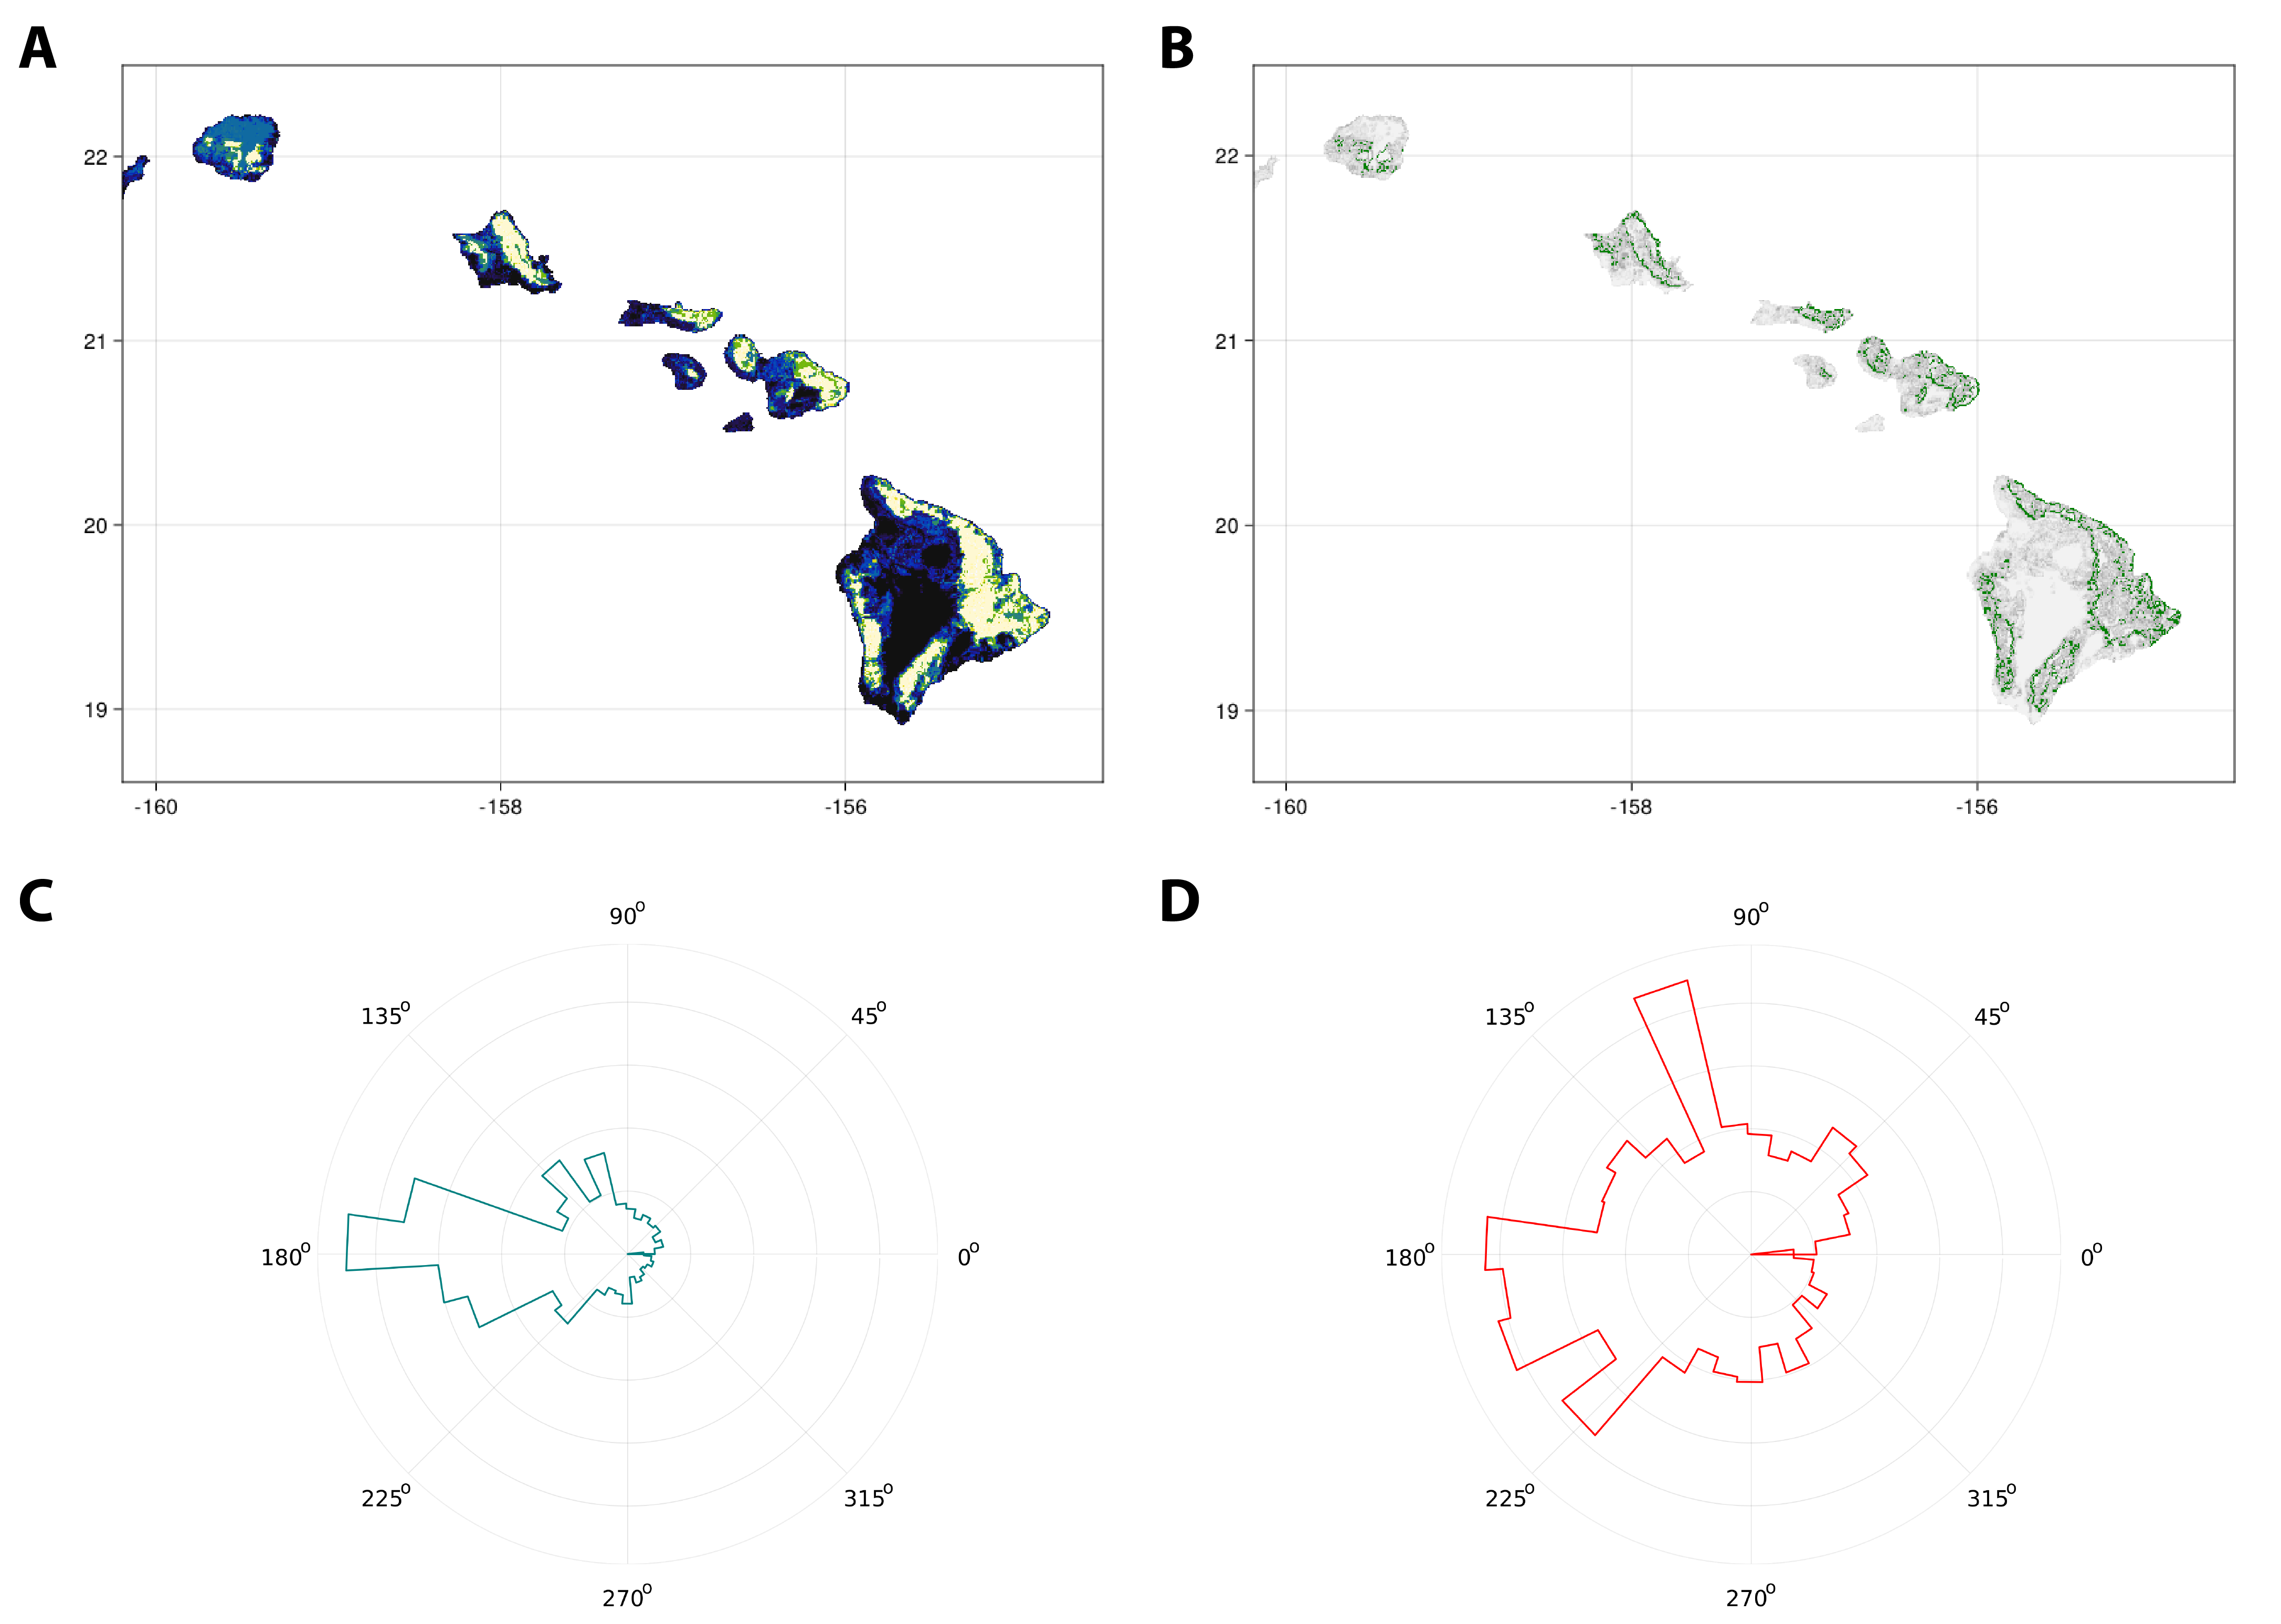
\includegraphics[width=\textwidth]{figures/fig_eg.png}
    \caption{\textbf{A} Woody plant coverage for Southwestern islands of the
Hawaiian Islands based on the sum of the cover for layers 1-4 from the
EarthEnv project. \textbf{B} the overall mean rate of change
(\emph{i.e.,} the composite of the wombled layers for layers 1-4) but
only for the cells identified as candidate boundary cells when using a
10\% threshold, with identified boundaries (shown in green) over the
rate of change (shown in levels of grey). The final two panels show the
direction of change for all cells (\textbf{C}) and only for cells
considered to be candidate boundary cells
(\textbf{D}).}
    \label{fig:example_womble}
\end{figure}

Although we have previously summed the four landcover layers for the
actual wombling part we will apply the wombling function to each layer
before we calculate the overall mean wombling value. We can broadcast
\texttt{wombling} in an element-wise fashion to the four different woody
cover layers. This will give as a vector containing four
\texttt{LatticeWomble} objects (since the input data was in the form of
a matrix).

\begin{verbatim}
wombled_layers = wombling.(lc[classes_with_trees])
\end{verbatim}

As we are interested in overall woody cover for Southwestern islands we
can take the \texttt{wombled\_layers} vector and use them with the
\texttt{mean} function to get the overall mean wombling value of the
rate and direction of change for woody cover. This will `flatten' the
four wombled layers into a single \texttt{LatticeWomble} object.

\begin{verbatim}
wombled_mean = mean(wombled_layers)
\end{verbatim}

From the \texttt{wombled\_mean} object we can `extract' the layers for
both the mean rate and direction of change. For ease of plotting we will
also convert these layers to \texttt{SimpleSDMPredictor} type objects.
It is also possible to call these matrices directly from the
\texttt{wombled\_mean} object, which has fields for \(m\) (the magnitude
of change) and \(\theta\) (the direction of change).

\begin{verbatim}
rate, direction = SimpleSDMPredictor(wombled_mean)
\end{verbatim}

Lastly we can identify candidate boundaries using the
\texttt{boundaries}. Here we will use a thresholding value (t) of 0.1
and save these candidate boundary cells as \texttt{b}. Note that we are
now working with a \texttt{SimpleSDMResponse} object and this is simply
for ease of plotting.

\begin{verbatim}
b = similar(rate)
b.grid[boundaries(wombled_mean, 0.1; ignorezero = true)] .= 1.0
\end{verbatim}

In addition to being used to help find candidate boundary cells we can
also use this object (\texttt{b}) as masking layer when visualising
wombling outputs. In this case we can view the \texttt{rate} layer in a
similar fashion to the original landcover layer but by masking it with
\texttt{b} we only plot the candidate boundaries (B in \autoref{fig:example_womble})
\emph{i.e.,} the cells with the top 10\% of highest rate of change
values. For visualisation we will overlay the identified boundaries (in
green) over the rate of change (in levels of grey)

\begin{verbatim}
heatmap(rate, colormap=[:grey95, :grey5])
heatmap!(b, colormap=[:transparent, :green])
current_figure()
\end{verbatim}

For this example we will plot the direction of change as radial plots
(third and fourth panels in \autoref{fig:example_womble}) to get an idea of the
prominent direction of change. Here we will plot \emph{all} the
direction values from \texttt{direction} for which the rate of change is
greater than zero (so as to avoid denoting directions for a slope that
does not exist) as well as the \texttt{direction} values from only
candidate cells using the same masking principle as what we did for the
rate of change. It is of course also possible to forgo the radial plots
and plot the direction of change in the same manner as the rate of
change should one wish.

Before we plot let us create our two `masked layers'. For all direction
values for which there is a corresponding rate of change greater than
zero we can use \texttt{rate} as a masking layer but first replace all
zero values with `nothing'. For the candidate boundary cells we can
simply mask \texttt{direction} with \texttt{b} as we did for the rate of
change.

\begin{verbatim}
direction_all = mask(replace(rate, 0 => nothing), direction)

direction_candidate = mask(b, direction)
\end{verbatim}

Because stephist() requires a vector of radians for plotting we must
first collect the cells and convert them from degrees to radians. Then
we can start by plotting the direction of change of \emph{all} cells (C
in \autoref{fig:example_womble}).

\begin{verbatim}
Plots.stephist(
         deg2rad.(values(direction_all));
         proj=:polar,
         lab="",
         c=:teal,
         nbins = 36,
         yshowaxis=false,
         normalize = false,
         dpi=600)
\end{verbatim}

Followed by plotting the direction of change only for cells that are
considered as candidate boundary cells (D in \autoref{fig:example_womble}).

\begin{verbatim}
Plots.stephist(
                deg2rad.(values(direction_candidate));
                proj=:polar,
                lab="",
                c=:red,
                nbins = 36,
                yshowaxis=false,
                normalize = false,
                dpi=600)
\end{verbatim}

\section{Summary}\label{summary}

Edge and boundary detection (as well as their delineation) is an
important and valuable concept in spatial ecology
(\cite{Cadenasso2003FraThe}) of which wombling serves as an approach that
is flexible in its execution (owing to the non-lattice or triangulation
capacity of the function) (\cite{Fortin2005SpaAna, Fortin1994EdgDet}) as
well as it's capacity to detect more nuanced landscape changes as
opposed to being limited to more abrupt discontinuities such as
cliffs/ridges by reducing noise in the landscape
(\cite{Matchev2020FinWom}). Wombling sets us up to answer two questions
about the geographic area of interest: at what rate and in which
direction does the variable of interest change? This of course has value
when it comes to evaluating the variation (or uniformity for that
matter) of a suite of ecological variables as well as how they may vary
with relation to each other.

\texttt{SpatialBoundaries.jl} provides the toolset with which to
implement both lattice and triangulation wombling using the
\texttt{wombling} function - multiple dispatch means that the structure
of the input dataset will determine exactly which algorithm is
implemented. This will simultaneously calculate both the rate and
direction of change and if desired multiple sets of different layers of
the same geographic area but defined by different
\(z\)-variables/surfaces can be aggregated and averaged to calculate the
overall mean wombling value. Both \texttt{wombling} and \texttt{mean}
will return objects of the type \texttt{Womble} of either the sub-type
\texttt{LatticeWomble} or \texttt{TriangulationWomble} depending on
which method was used. An object of any sub-type \texttt{Womble} can be
input into the \texttt{boundaries} function so as to identify cells that
can be considered as candidate boundaries based on a user specified
threshold.

\textbf{Acknowledgements:} We acknowledge that this study was conducted
on land within the traditional unceded territory of the Saint Lawrence
Iroquoian, Anishinabewaki, Mohawk, Huron-Wendat, and Omàmiwininiwak
nations. TS and TP are funded by a donation from the Courtois
Foundation.

\printbibliography{}
\end{refsection}

\endinput
%%